\section{辅助外设}
\subsection{微秒延时}
STM32的HAL库里提供了基于SysTick的延时函数\cinl{HAL_Delay(u32)},单位为毫秒。
但在我们的应用中,往往需要微秒级别的延时,例如ADS124S08的复位过程,
最小的$\overline{\text{RESET}}$引脚低电平持续时间为
$t_\textrm{w(RSL)} = 4\times t_\textrm{CLK}\approx\SI{1}{us}$.
因此我们需要借助定时器来实现微秒延时。

\subsubsection{基本定时器}
STM32H743拥有2个基本定时器,TIM6和TIM7,包含以下特性:

\begin{itemize}
    \item 16位自动重载递增计数器
    \item 16位可编程预分频器,用于对计数器时钟频率进行分频(可在运行时修改),
    分频系数介于1和65535之间
    \item 用于触发DAC的同步电路
    \item 发生如下更新事件时会生成中断/DMA请求:计数器上溢
\end{itemize}

由于我们只使用其计时功能,因此只需关注其时基单元:

\begin{itemize}
    \item 计数器寄存器 (TIMx\_CNT)
    \item 预分频器寄存器 (TIMx\_PSC)
    \item 自动重载寄存器 (TIMx\_ARR)
\end{itemize}

在自动重载寄存器(TIMx\_ARR)中添加一个计数值并使能TIMx后,计数寄存器(TIMx\_CNT)就会从0开始递增,
当TIMx\_CNT的数值与TIMx\_ARR值相同时就会生成事件并把TIMx\_CNT寄存器清0,完成一次循环过程。

注意,即使在计数器运行时,上述三个寄存器也可执行读写操作。因此我们可直接通过读取其寄存器判断是否
达到延时时间,而不需要使用事件中断。

\subsubsection{参数配置}
在STM32H7的时钟树上,我们可看到基本定时器TIM6/TIM7所在的APB1总线时钟是\SI{240}{MHz}:

\begin{figure}[H]
\center
    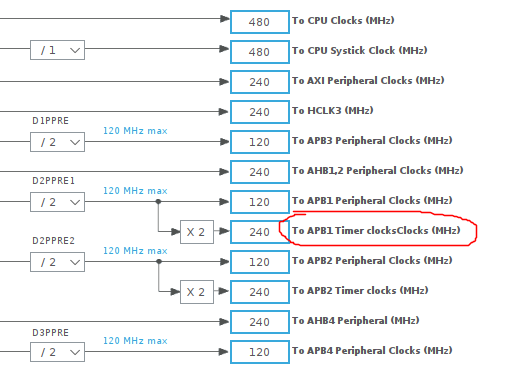
\includegraphics[width=0.8\textwidth]{img/tim6-clock.png}
    \captionof{figure}{外设总线时钟配置}
\end{figure}

为了达到微秒级别的延时,计数器预分频比不能超过$\SI{240}{MHz}\times\SI{1}{us}=240$.
由于我们的应用不需要较高的精度,因此为方便计算,直接设置预分频为240,
即让计数器工作在\SI{1}{MHz}的频率,每计数一次代表\SI{1}{ms}.
如果需要更精确的控制粒度,减小分频比即可。

计数器从0开始向上计到自动重载值(即TIMx\_ARR寄存器),然后重新从0开始计数并生成计数器上溢事件。
为了尽量提高可延时的范围,将自动重载值设到最大65535即可。

以下是基本定时器TIM6外设的最终配置:

\begin{figure}[H]
\center
    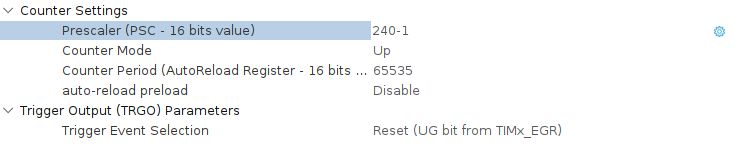
\includegraphics[width=\textwidth]{img/tim6-conf.png}
    \captionof{figure}{TIM6配置}
\end{figure}

注意:实际计数器工作时,会将配置的分频比加上1再参与计算,因此分频比应该配置为240-1.

\subsubsection{程序配置}

在前面的配置基础上,\cinl{delay_us}函数可简单实现如下:
\begin{cbox}{delay.h}
static INLINE
void delay_us(uint32_t us)
{
  /* 计数器值设置为0 */
  __HAL_TIM_SET_COUNTER(&htim6, 0);
  /* 等待计数器达到预定值 */
  while (__HAL_TIM_GET_COUNTER(&htim6) < us);
}
\end{cbox}

具体完整实现见文件\cinl{delay.h},这是一个header-only的库,其中实现了三个函数:

\begin{minted}{c}
static INLINE void delay_init();
static INLINE void delay_us(uint32_t us);
static INLINE void delay_ms(uint32_t ms);
\end{minted}

其中,\cinl{delay_init}负责使能TIM6;\cinl{delay_ms}则是对\cinl{HAL_Delay}的简单封装。
由于函数体都比较简单,因此函数全部声明为静态内联,避免函数调用带来的开销。

\subsection{GPIO Bundle操作}
在我们的应用中需要用到并口数据操作(AD9854),为了便于维护,在端口分配时尽量将同一组数据分配到
连续的几个GPIO口上,然后使用位运算统一操作。为此,定义GPIO组类型如下:

\begin{minted}{c}
typedef struct
{
  GPIO_TypeDef* port; /* GPIOx */
  uint8_t bits;       /* 位数 */
  uint8_t offset;     /* 偏移量 */
} gpio_group;
\end{minted}

为了能同时对多个GPIO引脚进行置位/清除,可以使用GPIOx\_BSRR寄存器,
查询STM32H7x3参考手册(RM0433)如下:

\begin{figure}[H]
\center
    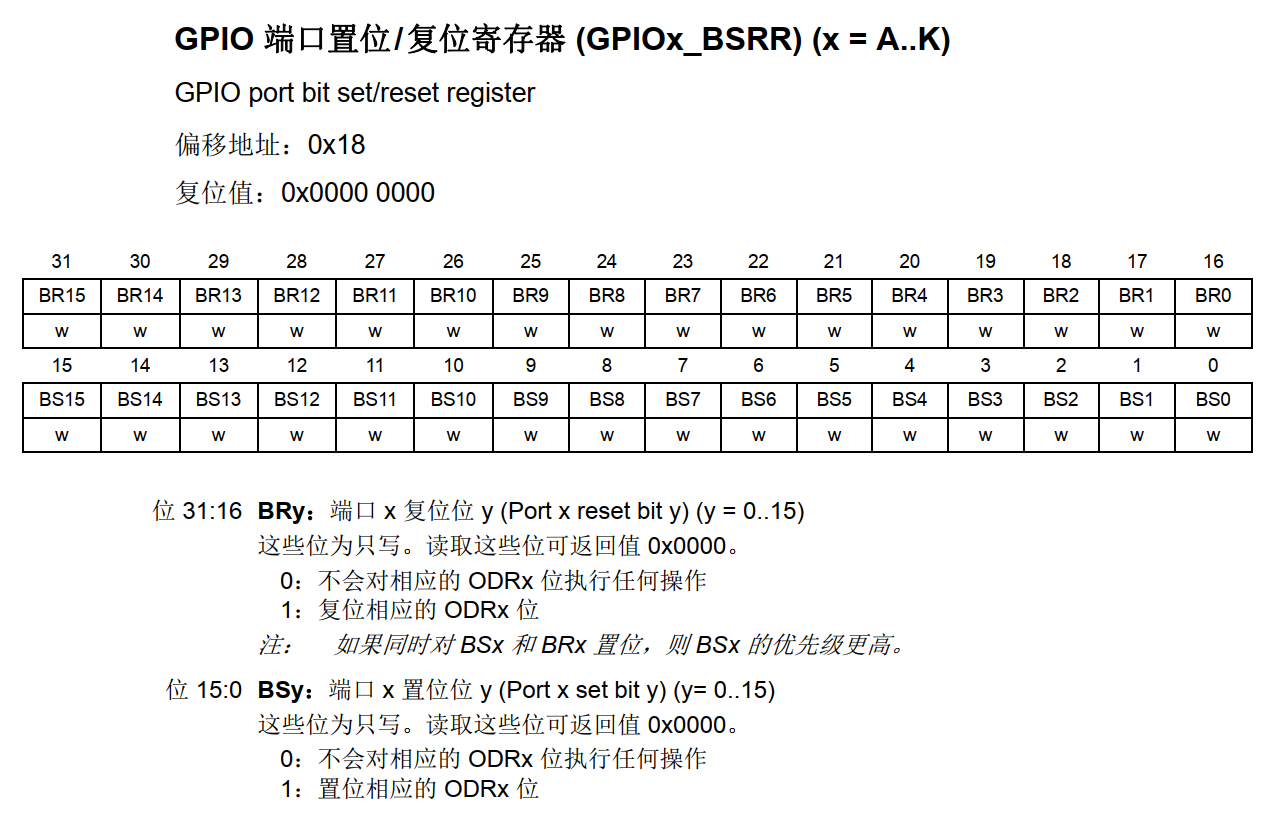
\includegraphics[width=\textwidth]{img/bsrr.png}
    \captionof{figure}{BSRR寄存器功能}
\end{figure}

通过同时设置BSRR寄存器的高16位和低16位,可以达到我们的要求:

\begin{cbox}{gpio\_wrapper.h}
static INLINE void
gpio_set_group(gpio_group group, uint16_t value)
{
  const uint16_t mask = ((uint16_t)1 << group.bits) - 1;
  group.port->BSRR = ((mask & value) | ((mask & ~value) << 16)) << group.offset;
}
\end{cbox}

我们先根据GPIO组的长度生成同样长度的掩码位,然后将数据和掩码相与,放入临时变量的低16位;
同时将数据取反的结果再和掩码相与,提取出需要清除的位,放入高16位,最后对结果取偏移,
得到BSRR寄存器的正确值。

使用类似的思路,可以编写GPIO组的读取函数:

\begin{cbox}{gpio\_wrapper.h}
static INLINE uint16_t
gpio_get_group(gpio_group group)
{
  const uint16_t mask = ((uint16_t)1 << group.bits) - 1;
  return mask & (group.port->IDR >> group.offset);
}
\end{cbox}
